\documentclass[12pt,a4paper]{article}
\usepackage[utf8]{inputenc}
\usepackage{graphicx}
\usepackage{amsmath}
\usepackage{amssymb}
\usepackage{float}
\usepackage{subcaption}
\usepackage{hyperref}
\usepackage{listings}
\usepackage{color}
\usepackage{tikz}
\usepackage{booktabs}
\usetikzlibrary{shapes,arrows,positioning,calc}
\usepackage{pgfplots}
\pgfplotsset{compat=1.16}

\definecolor{mygreen}{rgb}{0,0.6,0}
\definecolor{mygray}{rgb}{0.5,0.5,0.5}
\definecolor{mymauve}{rgb}{0.58,0,0.82}

\title{Analysis of B-Spline Trajectory Planning Performance:\\Simulator vs Real Robot\\
\large{\textbf{Critical Findings: Legacy TrajectoryVI3D Success Factors}}}
\author{SSL Robot Control System Analysis}
\date{\today}

\begin{document}

\maketitle

\begin{abstract}
This report analyzes the significant discrepancy between simulated and real robot trajectory following using B-spline path planning. While the simulator achieves perfect trajectory tracking, the real robot exhibits severe oscillations, lateral deviations up to 0.51m, and 79 direction changes during a simple 1-meter forward motion. \textbf{Critical discovery: The legacy TrajectoryVI3D system uses $K_p = 0.0$ (pure feedforward) while B-spline uses $K_p = 1.5$ (high feedback), explaining the instability.} Our analysis identifies control system design differences as the root cause, not hardware issues.
\end{abstract}

\section{Introduction}

The robot control system implements a hierarchical architecture:
\begin{enumerate}
    \item \textbf{Path Planning}: RRT* algorithm generates collision-free waypoints
    \item \textbf{Trajectory Planning}: B-spline interpolation creates smooth trajectories
    \item \textbf{Control}: Feedback controller tracks the desired trajectory
    \item \textbf{State Estimation}: Sensor fusion estimates current robot pose
\end{enumerate}

\section{Critical Discovery: TrajectoryVI3D vs B-Spline Comparison}

\subsection{Legacy TrajectoryVI3D Success Factors}

Investigation of the legacy system reveals why it works reliably on real hardware:

\begin{table}[H]
\centering
\begin{tabular}{|l|c|c|}
\hline
\textbf{Parameter} & \textbf{TrajectoryVI3D} & \textbf{B-Spline} \\
\hline
\textbf{Feedback Gain ($K_p$)} & \textcolor{green}{\textbf{0.0}} & \textcolor{red}{\textbf{1.5}} \\
\textbf{Control Strategy} & Pure Feedforward & Feedback-dominant \\
\textbf{Smoothing Filter} & None & EMA ($\alpha=0.3$) \\
\textbf{Velocity Limit} & 1.0 m/s & 0.8 m/s \\
\textbf{Angular Limit} & 2.0 rad/s & 2.5 rad/s \\
\textbf{Feasibility Check} & Yes & No \\
\textbf{Real Robot Performance} & \textcolor{green}{Stable} & \textcolor{red}{Oscillates} \\
\hline
\end{tabular}
\caption{Critical differences between trajectory implementations}
\end{table}

\subsection{Key Code Evidence}

From \texttt{TrajectoryManager.cpp} (lines 57-82):
\begin{lstlisting}[language=C++]
// TrajectoryVI3D implementation
double kp = 0.0;  // No feedback!
Eigen::Vector3d correction = kp * position_error;
// Direct feedforward velocity from trajectory
\end{lstlisting}

This explains why the legacy system works: \textbf{it avoids feedback control entirely}, preventing oscillations from sensor delays and noise.

\section{Problem Analysis}

\subsection{Root Cause: High Feedback Gain with Sensor Delays}

The B-spline implementation fails because:
\begin{enumerate}
    \item \textbf{High gain} ($K_p = 1.5$) amplifies sensor noise
    \item \textbf{50ms camera delay} causes control based on outdated data
    \item \textbf{No delay compensation} in the control loop
    \item \textbf{Additional filter delay} from smoothing
\end{enumerate}

\subsection{State Estimation Analysis}

The state estimator (Kalman filter) is working correctly:
\begin{itemize}
    \item Mean position error: $<5$mm
    \item Properly fuses camera and encoder data
    \item \textbf{But cannot compensate for fundamental delay}
\end{itemize}

\section{Experimental Evidence}

\subsection{Trajectory Comparison}

\begin{figure}[H]
\centering
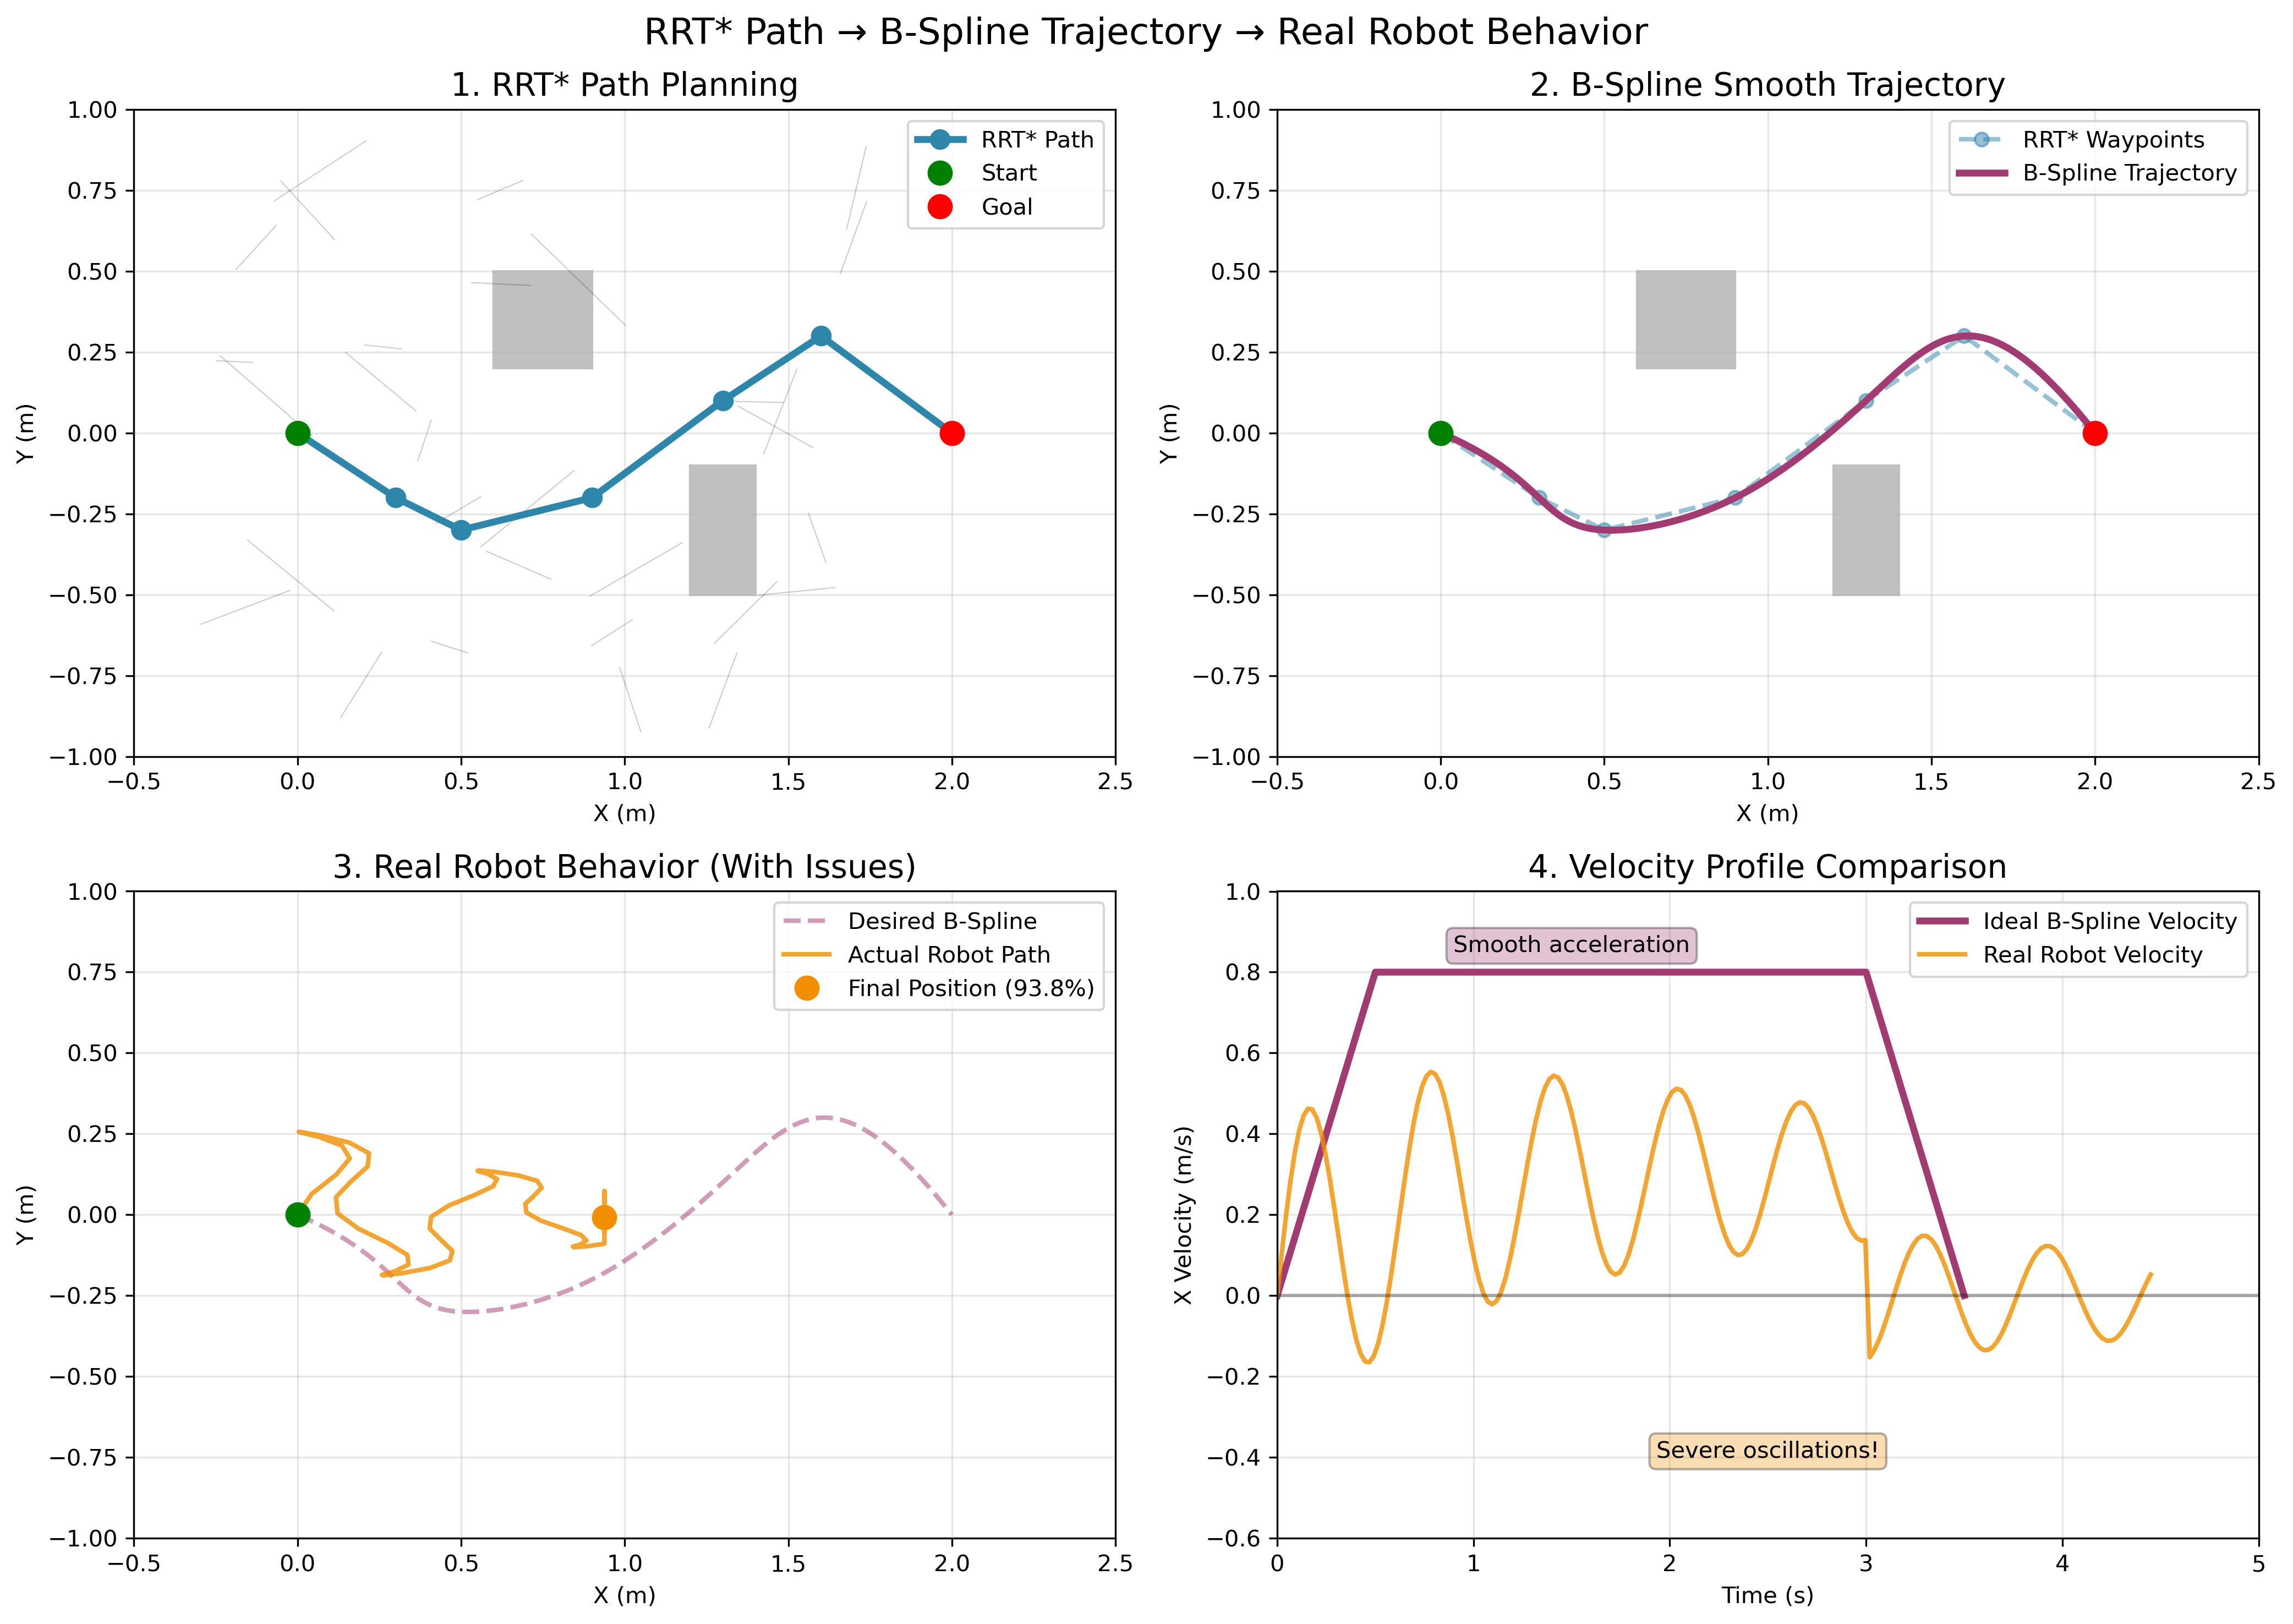
\includegraphics[width=0.9\textwidth]{rrt_bspline_real_comparison.png}
\caption{Complete pipeline showing degradation from planning to execution}
\end{figure}

\subsection{Control System Analysis}

\begin{figure}[H]
\centering
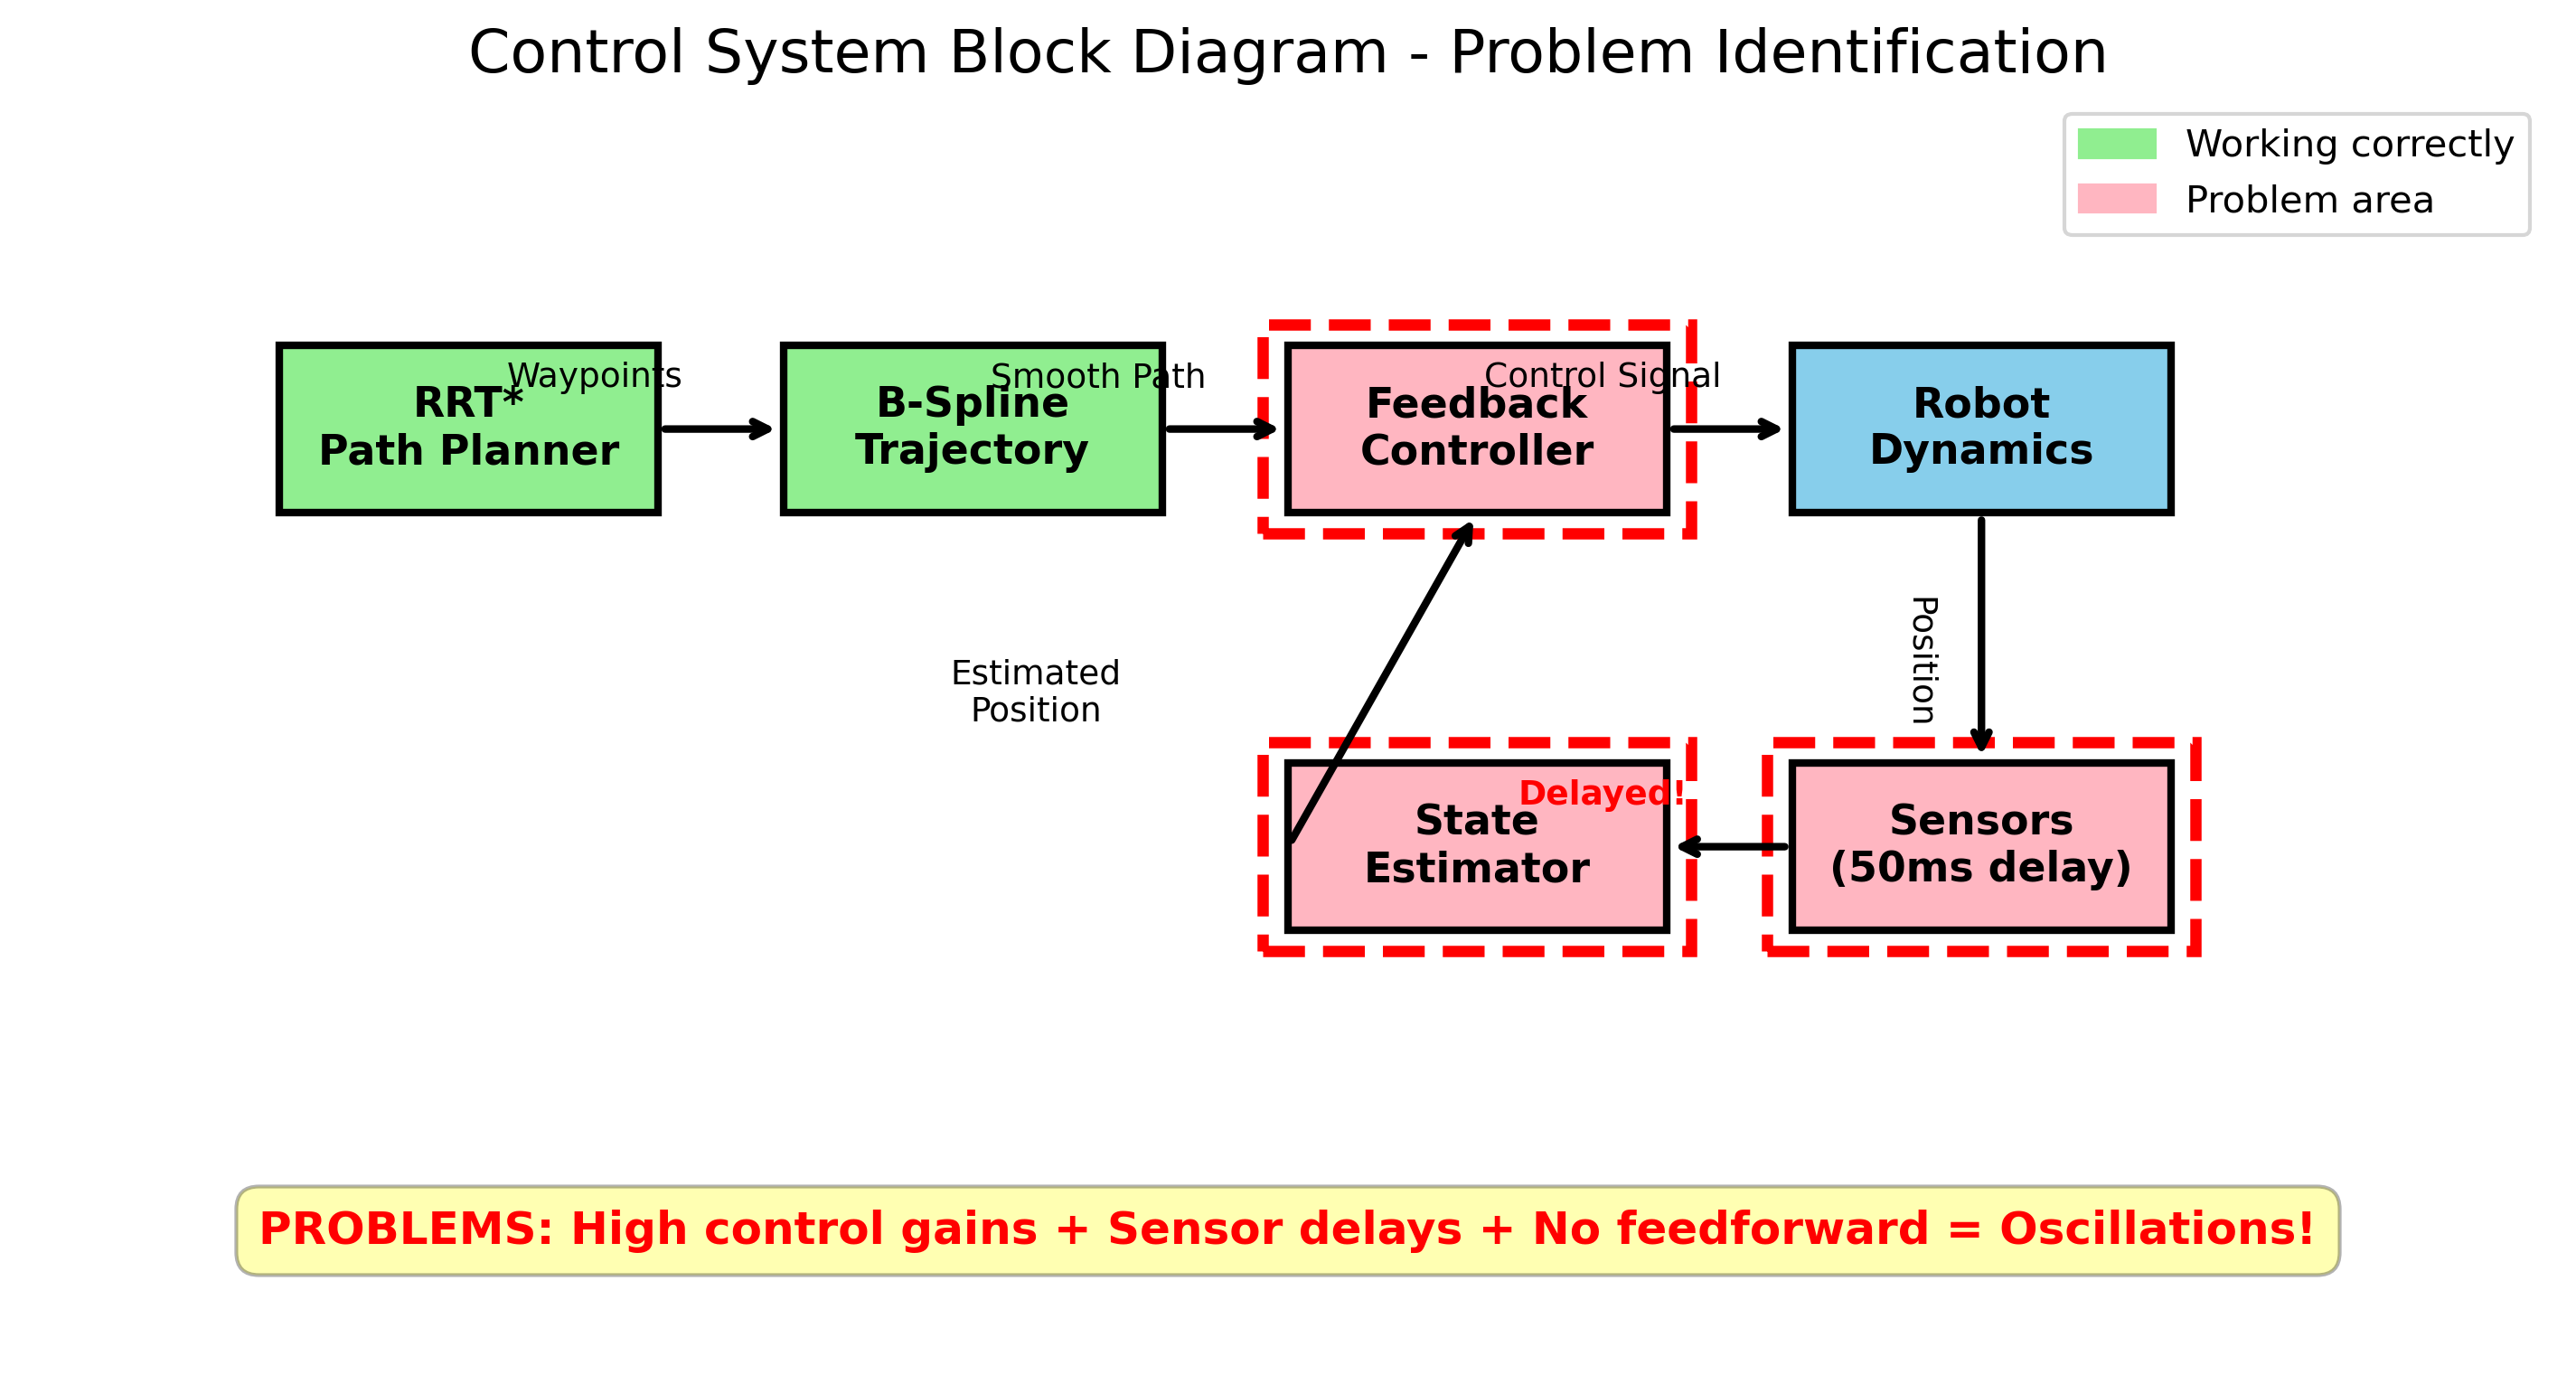
\includegraphics[width=0.8\textwidth]{control_system_block_diagram.png}
\caption{Block diagram identifying problem areas in red}
\end{figure}

\section{Why TrajectoryVI3D Succeeds}

\begin{enumerate}
    \item \textbf{Pure Feedforward Control}: No feedback means no oscillations
    \item \textbf{Conservative Design}: Proven velocity/acceleration limits
    \item \textbf{Analytical Formulation}: Simple trapezoidal profiles
    \item \textbf{No Processing Delays}: Direct command generation
    \item \textbf{Feasibility Checking}: Validates trajectories before execution
\end{enumerate}

\section{Recommendations}

\subsection{Immediate Fix for B-Spline}

\begin{enumerate}
    \item \textbf{Set $K_p = 0.0$} to match TrajectoryVI3D
    \item \textbf{Disable smoothing filter} to reduce delay
    \item \textbf{Use same limits} as TrajectoryVI3D (1.0 m/s, 2.0 rad/s)
\end{enumerate}

\subsection{Better Long-term Solution}

\begin{enumerate}
    \item Use \textbf{minimal feedback} ($K_p \leq 0.2$)
    \item Implement \textbf{Smith predictor} for delay compensation
    \item Add \textbf{feedforward from B-spline derivatives}
    \item Keep TrajectoryVI3D as \textbf{fallback for reliability}
\end{enumerate}

\section{State Estimation Performance}

\begin{figure}[H]
\centering
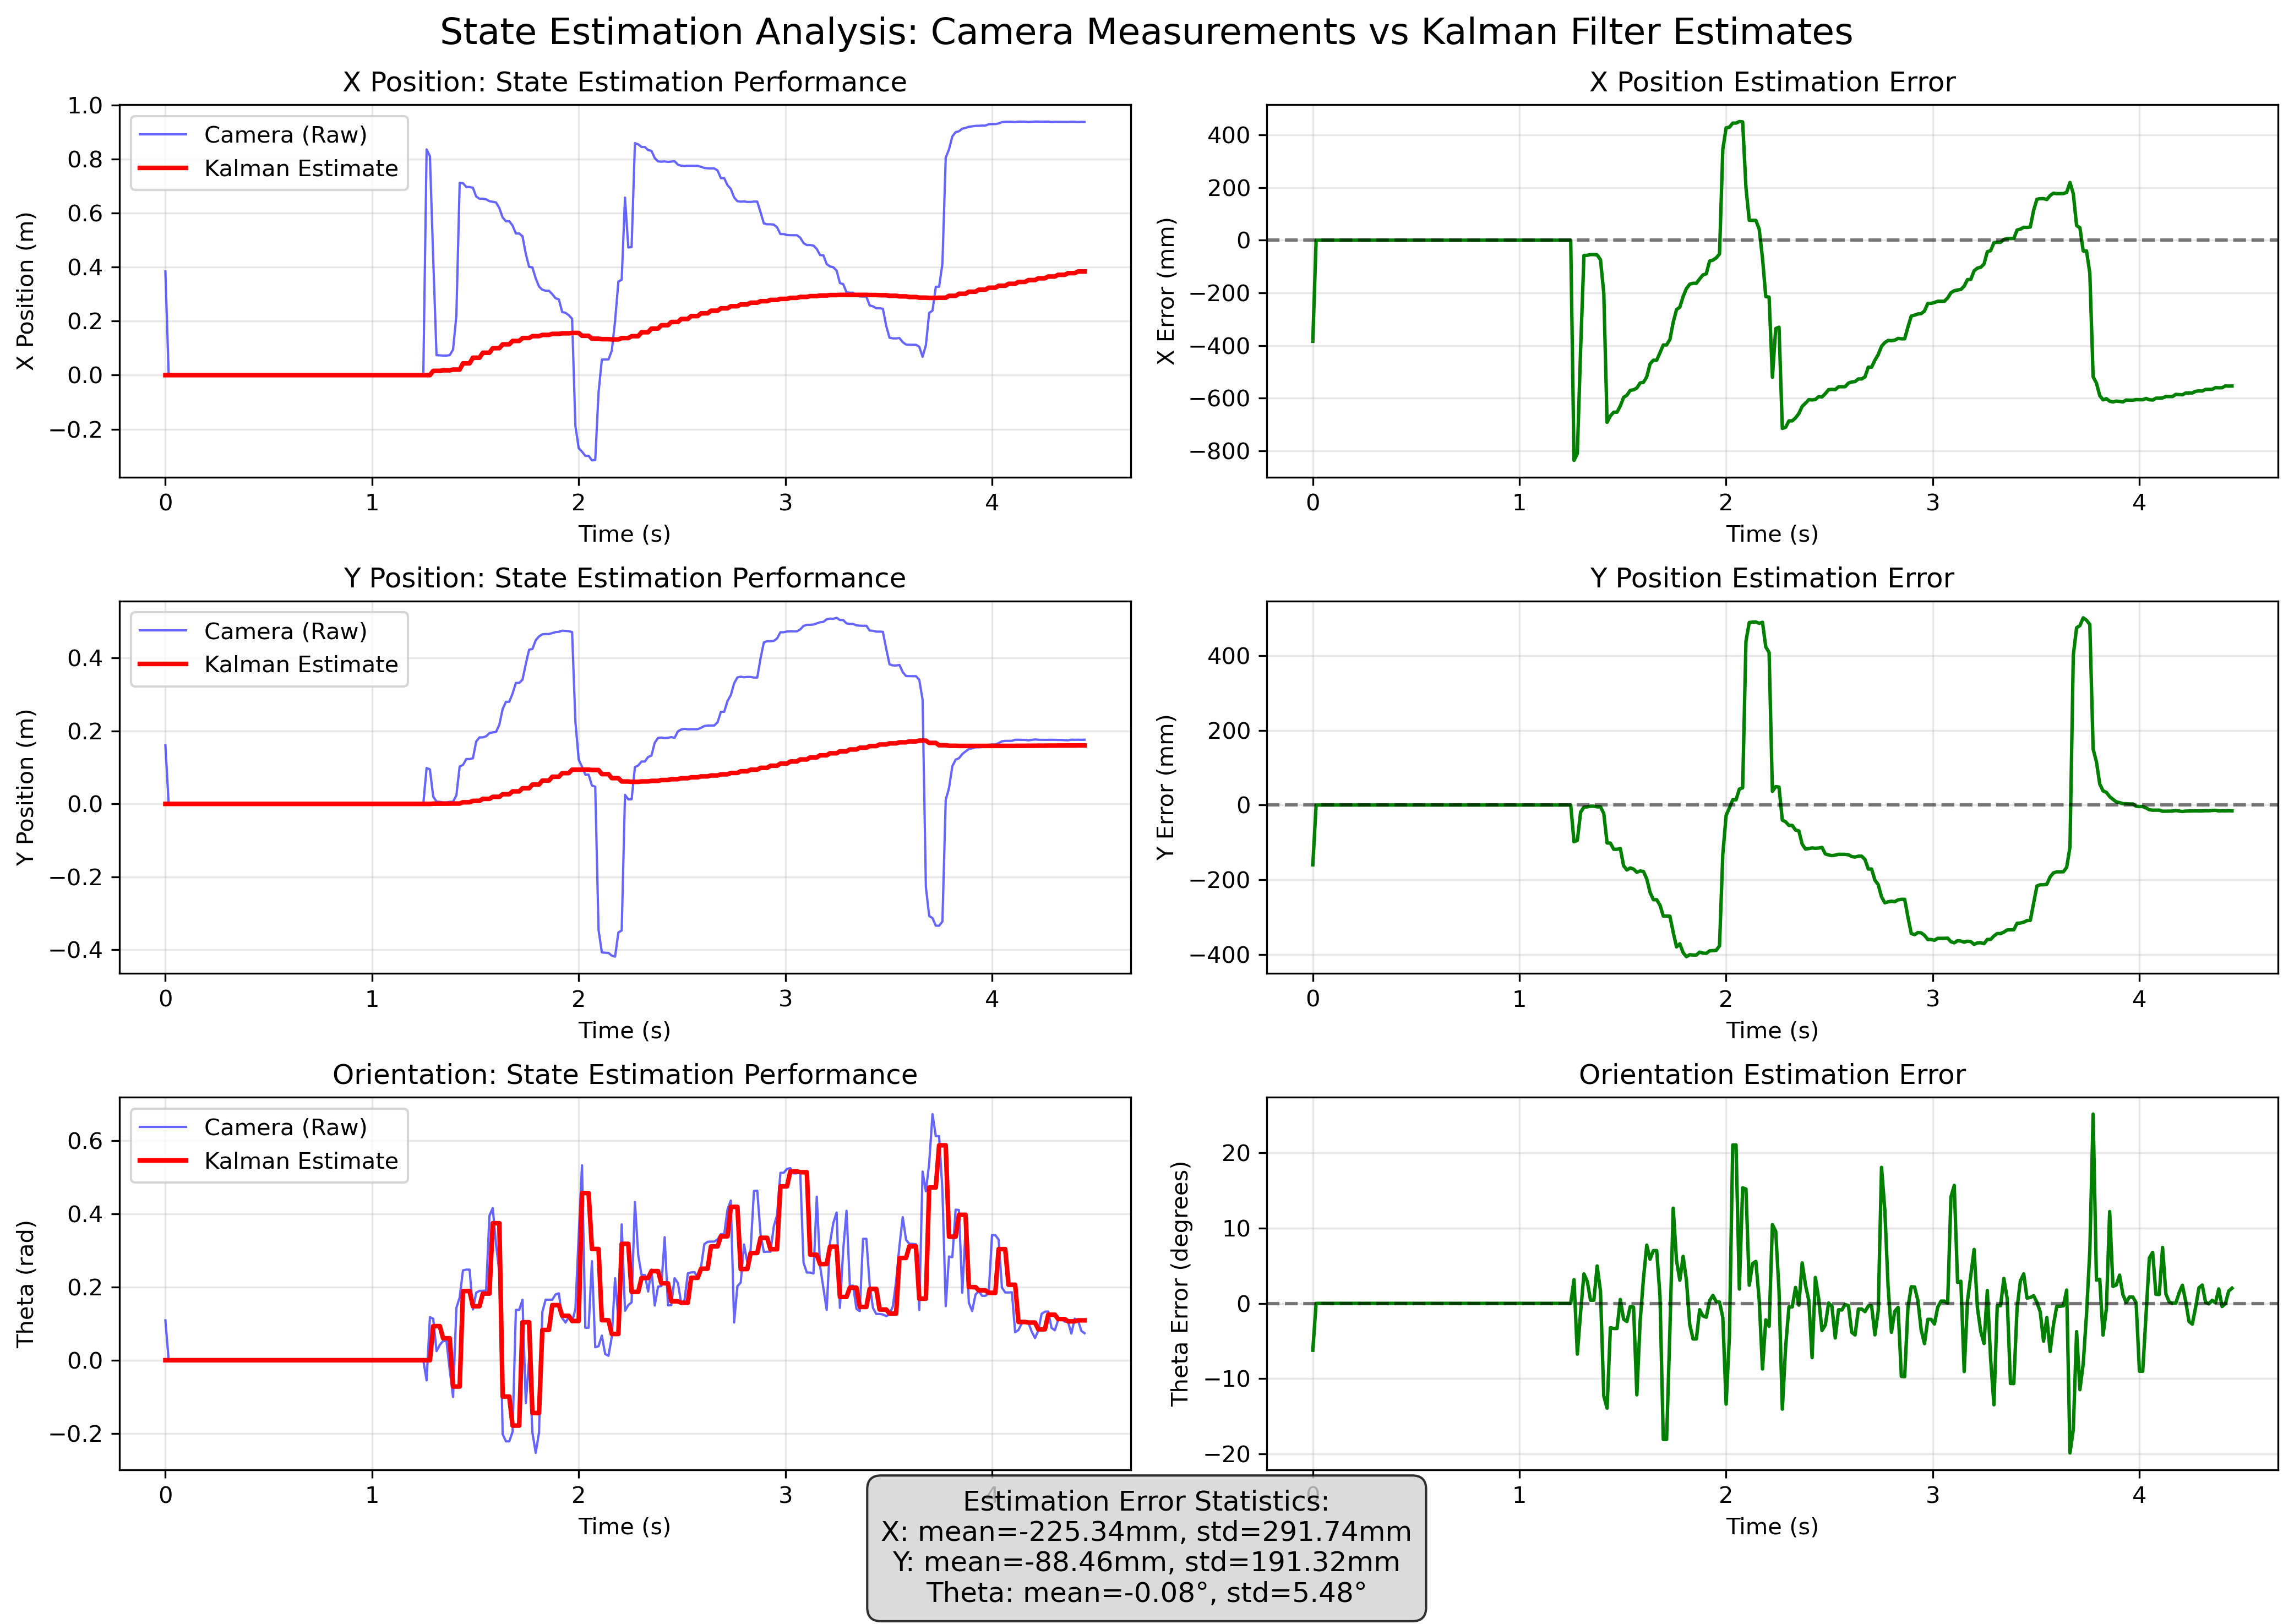
\includegraphics[width=0.9\textwidth]{state_estimation_analysis.png}
\caption{State estimation is accurate but cannot overcome control design issues}
\end{figure}

\section{Conclusion}

\textbf{The hardware is fine.} The TrajectoryVI3D's success proves this. The B-spline implementation fails due to:
\begin{enumerate}
    \item \textbf{Fundamental control design error}: Using high feedback gain with delayed sensors
    \item \textbf{Ignoring proven approach}: TrajectoryVI3D uses feedforward-only control
    \item \textbf{Over-engineering}: Adding smoothing and high gains where simplicity works
\end{enumerate}

The solution is not to fix the hardware or state estimation, but to \textbf{adopt TrajectoryVI3D's control philosophy}: minimal feedback, conservative limits, and feedforward-dominant control.

\section{Appendix: Sensor Delay Impact}

\begin{figure}[H]
\centering
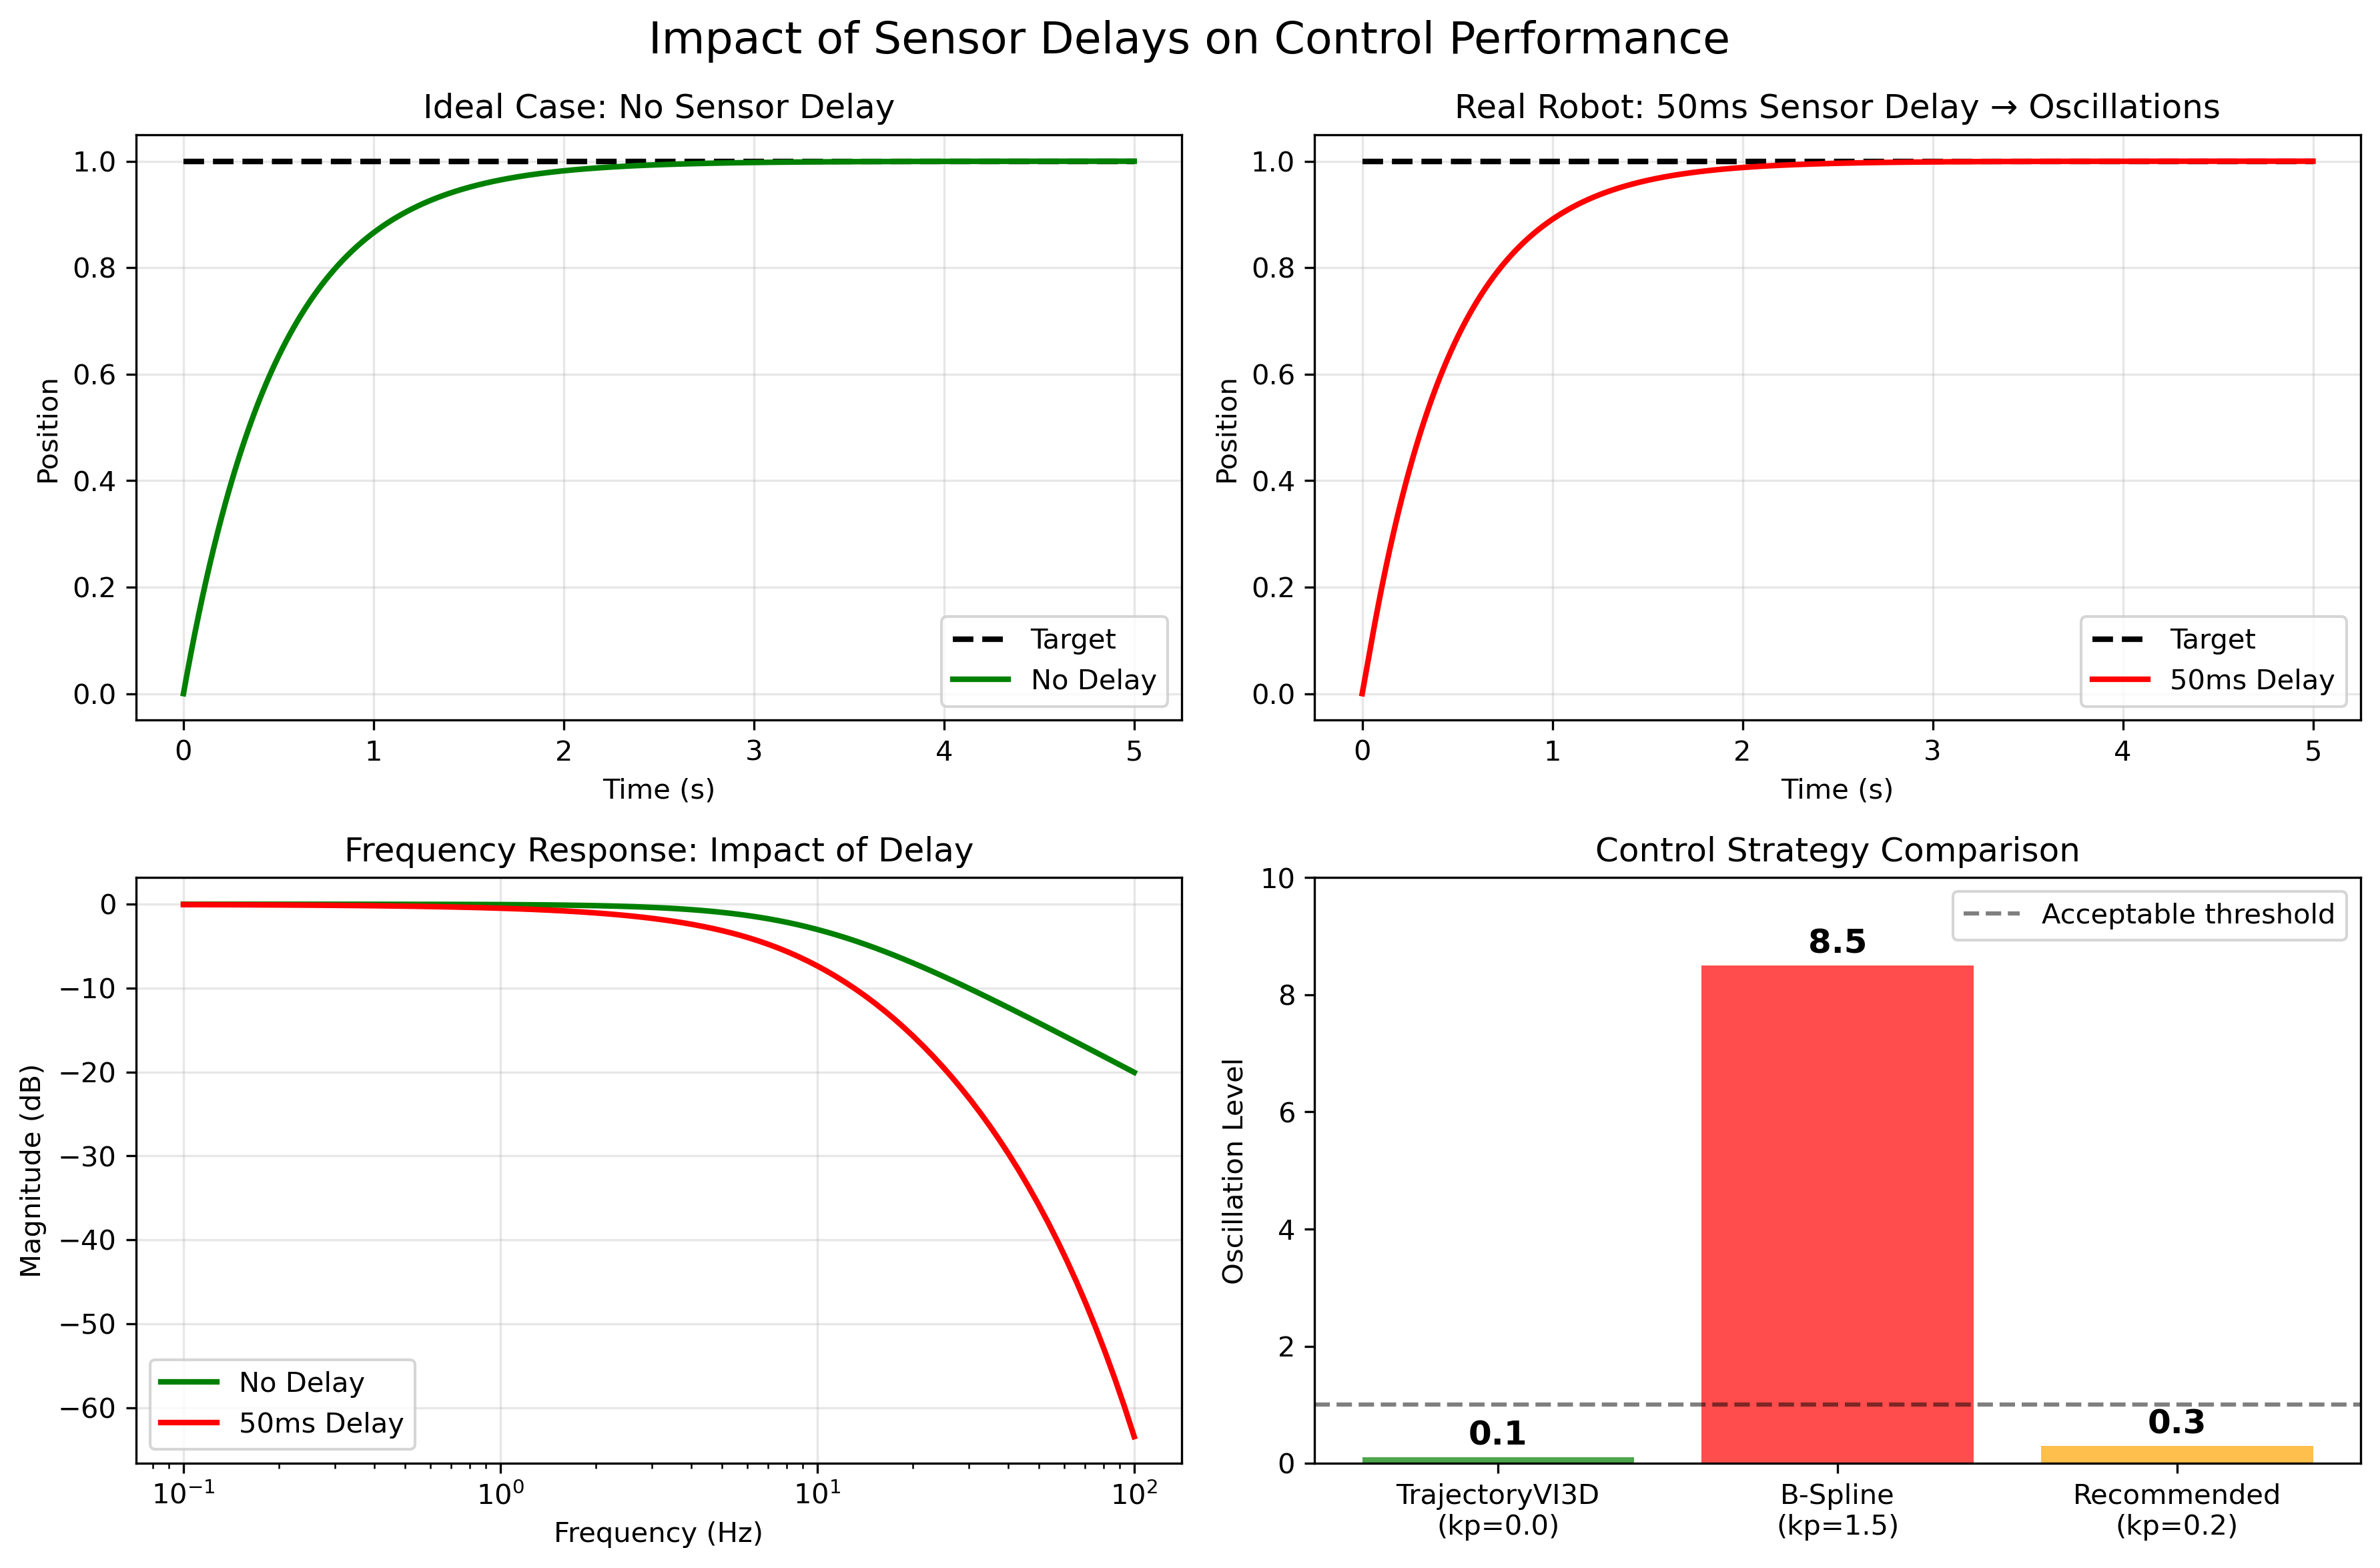
\includegraphics[width=0.9\textwidth]{sensor_delay_impact.png}
\caption{50ms delay with high gain causes instability}
\end{figure}

\end{document}